% -*-latex-*-
%\documentclass[handout]{beamer} 
\documentclass[]{beamer} 
\usepackage{etex}
\title{Neolithic Adaptations}
\author{Alan R. Rogers}
\date{\today}
\begin{document}

\frame{\titlepage}

\begin{frame}
\frametitle{Outline}
\begin{itemize}
\item Lactase persistence
\item Skin color
\item Molecular archaeology
\end{itemize}
\end{frame}

\begin{frame}
\frametitle{The trouble with fresh milk}
\begin{itemize}
\item Contains the sugar \emph{lactose}
\item Digesting lactose requires the enzyme \emph{lactase}
\item Most humans don't produce it after age 5.
\item Fresh milk gives them gas and diarrhea.
\item 8000 years ago, all humans had this problem.
\end{itemize}
\end{frame}

\begin{frame}
\frametitle{Lactase persistence}
\begin{itemize}
\item Some modern humans produce lactase throughout life.
\item Digest fresh milk as adults.
\item Caused by mutation near lactase gene.
\item When and where?
\end{itemize}
\end{frame}

\begin{frame}
\frametitle{Distribution of lactase persistence (dark blue)}
 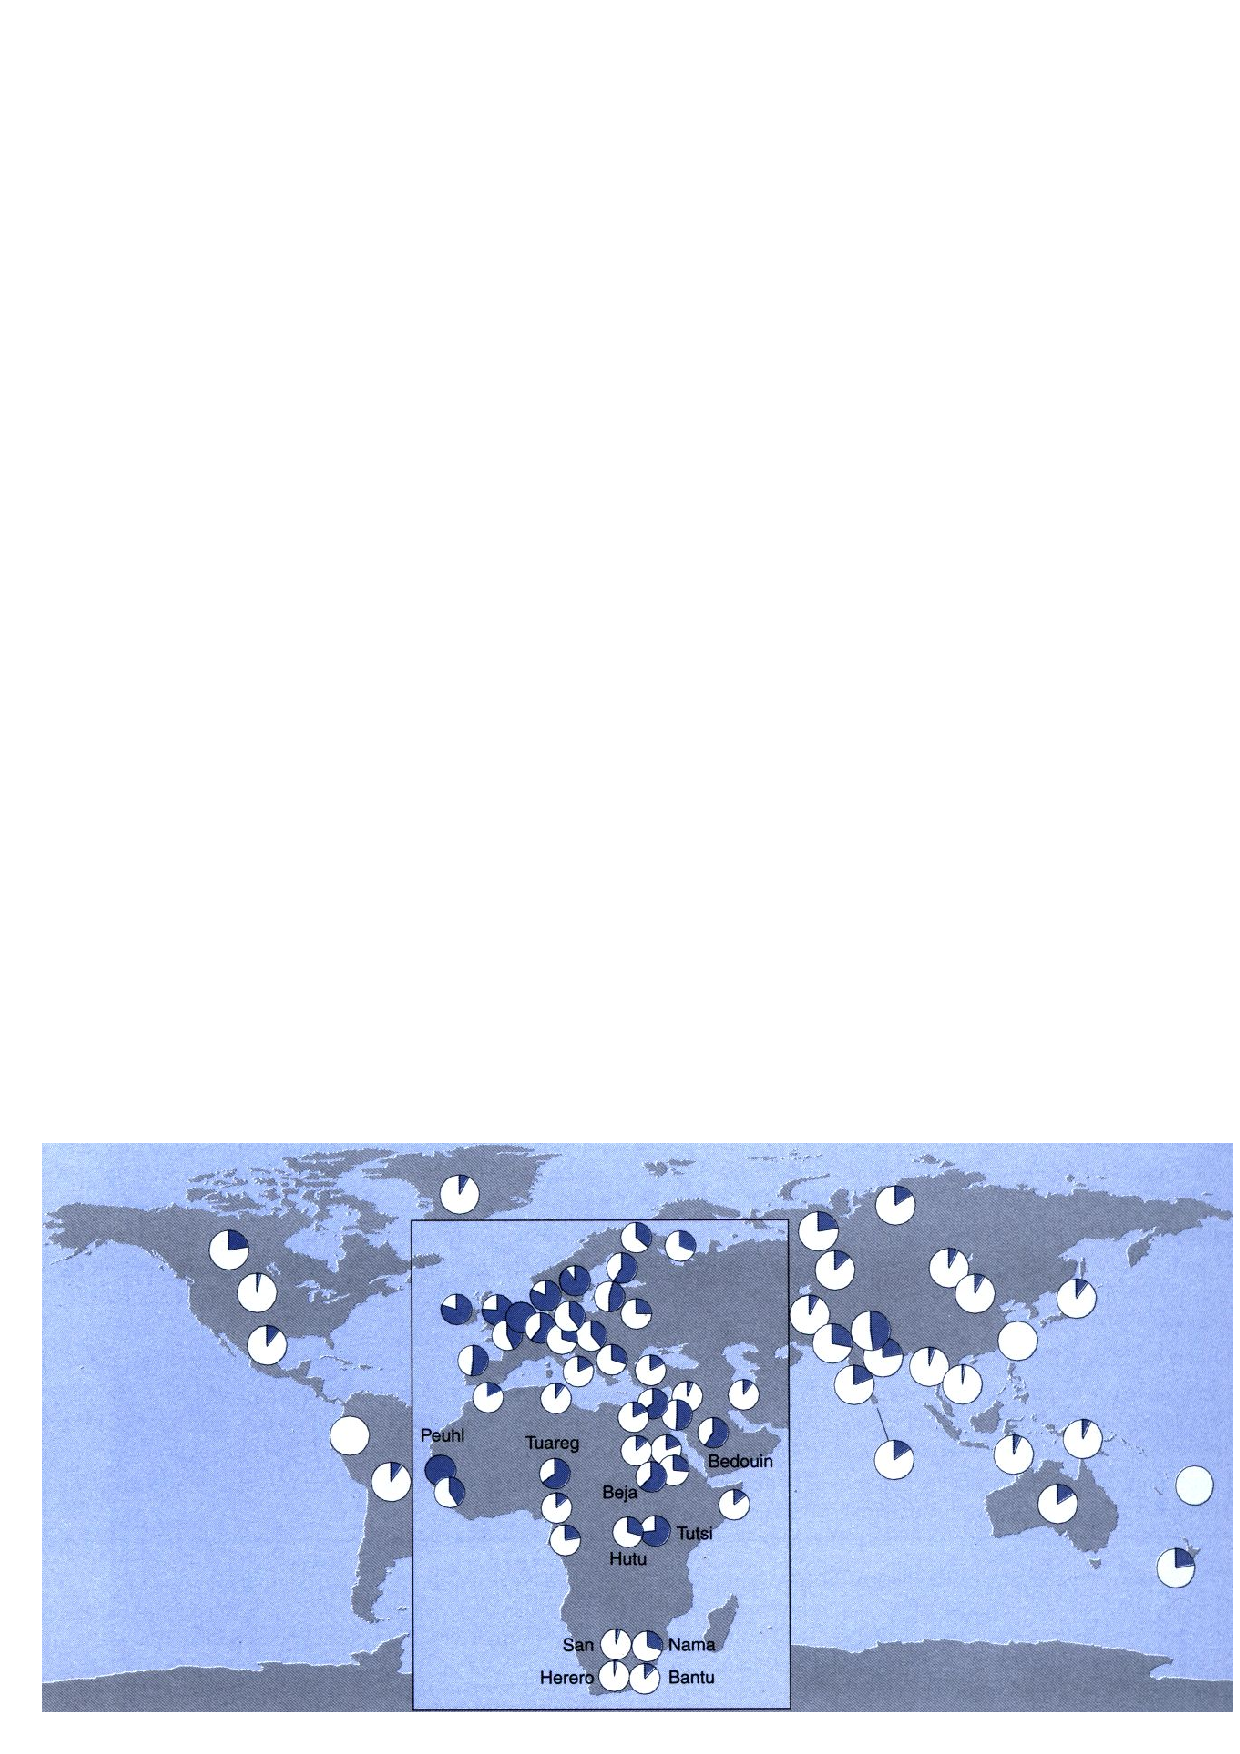
\includegraphics[width=\textwidth]{lacmap.pdf}
\end{frame}

\begin{frame}
\frametitle{Within countries, lactase persistence more common in
 populations that drink milk}
 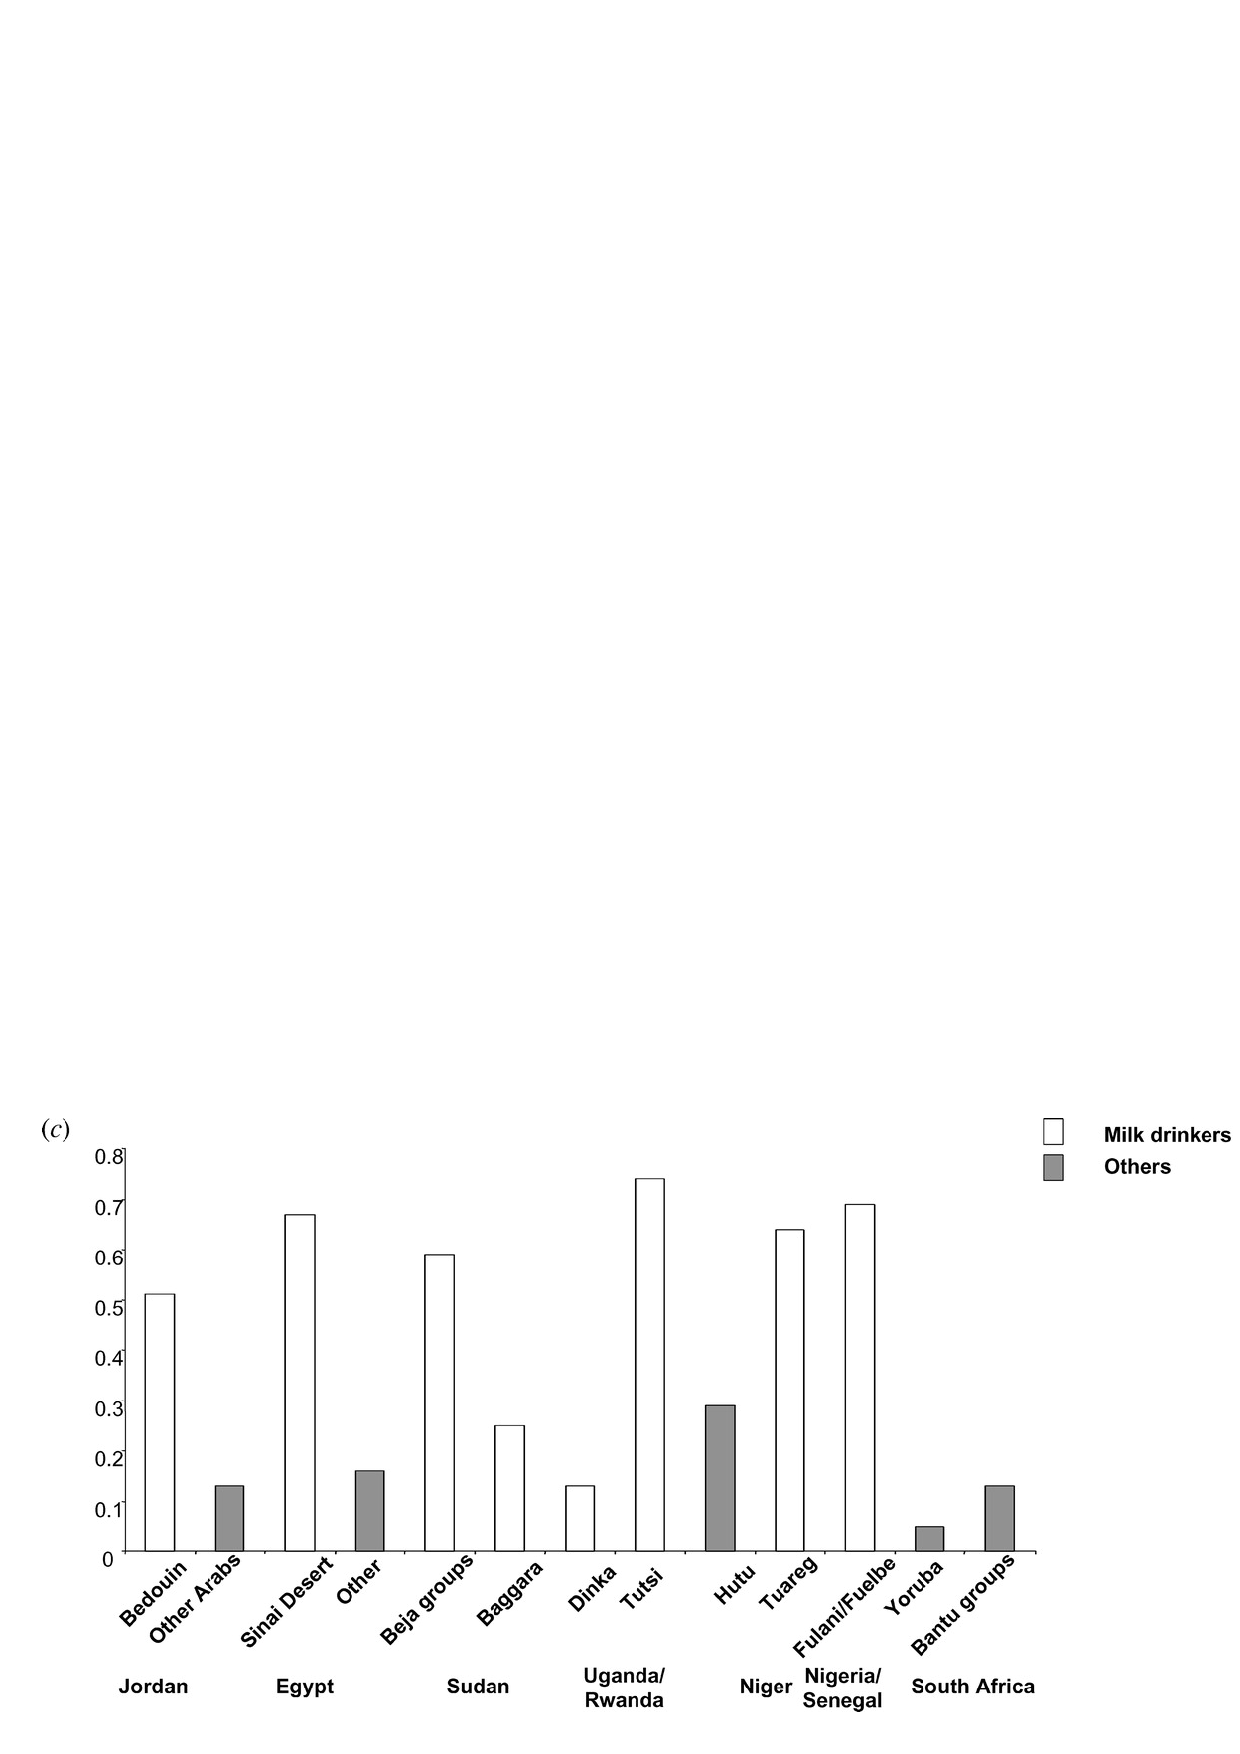
\includegraphics[width=\textwidth]{lacdiet.pdf}
\end{frame}

\begin{frame}
\frametitle{Evidence for a selective sweep}
\begin{itemize}
\item In Europeans, persistence allele surrounded by a million bases
  of LD.
\item Indicates strong selection.
\item Statistical tests reject the drift hypothesis (Bersaglieri et al
      2004)
\item Increasing for $\sim$10,000 years (Coelho et al 2005).
\end{itemize}
\end{frame}

\begin{frame}
\frametitle{LD surrounds lactase gene in Europe}
 \includegraphics[width=\textwidth]{voigt-loci.pdf}
\end{frame}

\begin{frame}
\frametitle{Huge block of LD around lactase allele in Europe}
{\centering\includegraphics[width=\textwidth]{lac.png}\\}
\mbox{}\hfill\small (Nathan Harris)\\
\end{frame}

\begin{frame}
\begin{columns}
\column{0.7\textwidth}
\fbox{\includegraphics[height=0.9\textheight]{coelho.pdf}}
\column{0.35\textwidth}
\raggedright
\begin{itemize}
\item Rows are different STRs
\item Lactase persistence allele: haplotype TA.
\item Has reduced SNP variation,
\item Indicates recent origin.
\item Age: 7,450 or 12,300 years (depending on assumptions)
\end{itemize}
\end{columns}
\end{frame}

\begin{frame}
\frametitle{Outline}
\begin{itemize}
\item[$\circ$] Lactase persistence
\item Skin color
\item Molecular archaeology
\end{itemize}
\end{frame}

\begin{frame}
\begin{columns}
\column{0.7\textwidth}
\includegraphics[width=\linewidth]{CapeVerde-map.png}
\column{0.3\textwidth}
\textcolor{blue}{\large Cape Verde Islands}

\bigskip

A good place to study genetic variation in skin color.
\end{columns}
\end{frame}

\begin{frame}
\frametitle{Why Cape Verde is ideal}
\begin{columns}
\column{0.5\textwidth}
\includegraphics[width=\linewidth]{Beleza-histogram.png}
\column{0.5\textwidth}
Population is close to a 50:50 mixture of African and European
ancestry.  

\bigskip

Lots of variation at loci that differ between the continents.

\bigskip

African Americans (dotted lines) are much more African.
\end{columns}
\end{frame}

\begin{frame}
\includegraphics[width=\linewidth]{CapeVerde-sports.jpg}
\end{frame}

\begin{frame}
\frametitle{Genome-wide association study (GWAS) of skin color}
\begin{columns}
\column{0.5\textwidth}
\includegraphics[width=\linewidth]{Beleza-map.png}
\column{0.5\textwidth}
\begin{itemize}
\item GWAS: look for loci associated with skin color
\item Beleza et al (2013).
\end{itemize}
\end{columns}
\end{frame}

\begin{frame}
\frametitle{Locus SLC24A5 affects skin color}
\includegraphics[width=\linewidth]{Beleza-GWAS-skincolor.png}
\end{frame}

\begin{frame}
\frametitle{3 other loci pop out after adjusting for SLC24A5}
\includegraphics[width=\linewidth]{Beleza-GWAS2-skincolor.png}
\end{frame}

\begin{frame}
\frametitle{Locus HERC2 affects eye color}
\includegraphics[width=\linewidth]{Beleza-GWAS-eyecolor.png}
\end{frame}

\begin{frame}
\frametitle{SLC24A5 affects eyes as well as skin}
\includegraphics[width=\linewidth]{Beleza-GWAS2-eyecolor.png}
\end{frame}

\begin{frame}
\frametitle{Outline}
\begin{itemize}
\item[$\circ$] Lactase persistence
\item[$\circ$] Skin color
\item Molecular archaeology
\end{itemize}
\end{frame}

\begin{frame}
\frametitle{Postglacial History of Europe}
\begin{description}
\item[12~kya] Warm Post-glacial climate. Europe inhabited by
  Mesolithic foragers.
\item[7~kya] Neolithic: farmers expand into Europe from Middle East
  and Anatolia, largely replacing foragers.
\item[5~kya] Pastoralists invade Europe from Russia and Ukraine,
  largely replacing early Neolithic peoples (especially the males). 
\end{description}
\end{frame}

\begin{frame}
\frametitle{La Bra{\~n}a, a 7000-y-old Mesolithic European}
\begin{columns}
\column{0.5\textwidth}
\includegraphics[width=\linewidth]{LaBrana-map.png}
\column{0.5\textwidth}
\includegraphics[width=\linewidth]{LaBrana-bones.jpg}
\end{columns}
\end{frame}

\begin{frame}
\frametitle{Mesolithic Europeans: dark skin \& blue eyes}
\begin{columns}
\column{0.5\textwidth}
\includegraphics[width=\linewidth]{mesolithicFace.jpg}
\column{0.5\textwidth}
\textcolor{blue}{Dark skin:} Ancestral (dark-skin) allele at SLC45A2,
SLC24A5, MC1R, TYR and KITLG.  Derived (light-skin) alleles at TYRP1,
ASIP and IRF4.

\bigskip

\textcolor{blue}{Blue eyes:} Derived (blue-eye) allele at HERC2.
\end{columns}
\end{frame}

\begin{frame}
\frametitle{Study of Mathieson et al 2015}
\begin{itemize}
\item DNA from 83 ancient Europeans.
\item Track changes in allele frequencies over time.
\end{itemize}
\end{frame}

\begin{frame}
\frametitle{History of evolution in Europe}
\includegraphics[width=\linewidth]{Mathieson-allele-hist.png}\\
\textcolor{blue}{Eye color} Blue eyes early; brown with Neolithic;
blue comes back 4~kya.\\

\medskip

\textcolor{blue}{Skin color} Dark early; lighter with Neolithic;
lighter still 4~kya.
\end{frame}

\begin{frame}
\frametitle{History of evolution in Europe}
\includegraphics[width=\linewidth]{Mathieson-allele-hist.png}\\

\bigskip

\textcolor{violet}{Lactase persistence begins in Europe around 4000~BP.} \\
\end{frame}

\begin{frame}
  \frametitle{Comparing Neolithic Europeans with their Anatolian
    Ancestors}
  The Neolithic begins in the Middle East and Anatolia (modern Turkey)
  about 7000~ya.

  \bigskip

  One axis of spread went north into the Danube basin and then west
  into Germany and France.

  \bigskip

  Early farmers of this northern region: the ``Linearbandkeramik (LBK)
  culture''.

  \bigskip
  
  Childebayeva et al (2022) compared LBK farmers earlier Anatolian farmers.
\end{frame}

\begin{frame}
  \includegraphics[width=\textwidth]{Childebayeva-pca-map-struc.png}
\end{frame}

\begin{frame}
  \includegraphics[width=\textwidth]{Childebayeva-seln.png}
\end{frame}

\begin{frame}
\frametitle{Summary}
\begin{itemize}
\item Mesolithic foragers were dark, with blue eyes; lactose intolerant.
\item Neolithic brought lighter skin and dark eyes; still lactose
  intolerant. 
\item Indo-Europeans brought lighter skin, blue eyes, maybe lactase
  persistence. 
\item Frequency of lactase persistence increases after 4~kya.
\end{itemize}
\end{frame}

\end{document}
